% Chapter 4

\chapter{Methodology} % Main chapter title

\label{Chapter4} % For referencing the chapter elsewhere, use \ref{Chapter4}

%----------------------------------------------------------------------------------------

\section{Data preprocessing}

This study is based on the interpretation of wind and wave conditions using in situ and remote sensing observations from buoys and altimeters. There are fundamental differences in how in situ platforms measure and report the geophysical parameters compared to observations from satellite altimeters. On the one hand, buoys' measurements are considered the "ground truth", owing to their ability to provide a reliable, long-term, and continuous time-series record of temporally processed oceanographic and meteorological parameters from the raw data for a specific location. On the other hand, altimeters provide instantaneous measurements representing their sea surface footprint with a low temporal resolution. A description of satellite coastal altimetry challenges is available in \ref{AltimetryPrinciples}. 

This chapter aims to provide an outline of the collection and preprocess of the different data types. This step is essential because both datasets contain inherent and unique sources of error \cite{Glazman1990, Monaldo1988, Zieger2009}, and they need to be quality controlled before the analysis. The next step is to accurately describe the methodology that was implemented to achieve our final results. 


%-------------------------------------------------------------------------------------------


\subsection{Buoy Data Collection and Organization}\label{buoy_observations}

The importance of an extended and well-preserved network of buoys in the United States of America is well documented in \cite{Castellini2011}. This study utilizes all the wind and wave geophysical parameters reported by multiple stations of the NDBC and CDIP. CDIP is operated by the Ocean Engineering Research Group (OERG), part of the Integrative Oceanography Division (IOD) at Scripps Institution of Oceanography (SIO), and it is responsible for the operation and maintenance of buoys 44097 and 44091. Buoy 44039 is part of the Long Island Sound Integrated Coastal Observing System (LISICOS), and it is operated and maintained by the University of Connecticut (UConn) Marine Sciences Department. The remaining buoys are operated and maintained by NDBC.


\begin{figure}
    \centering
    \subfloat[\centering Buoy 44025 (Long Island) ]{{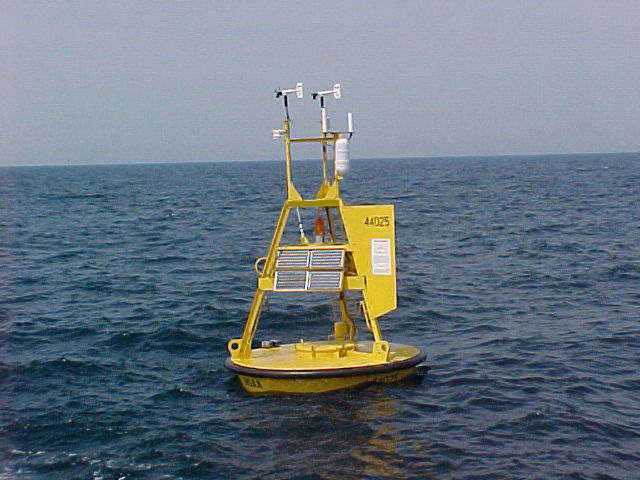
\includegraphics[height=6cm]{Figures/Chapter4/NDBCbuoy.jpg} }}%
    \qquad
    \subfloat[\centering CDIP Datawell Waverider Buoy ]{{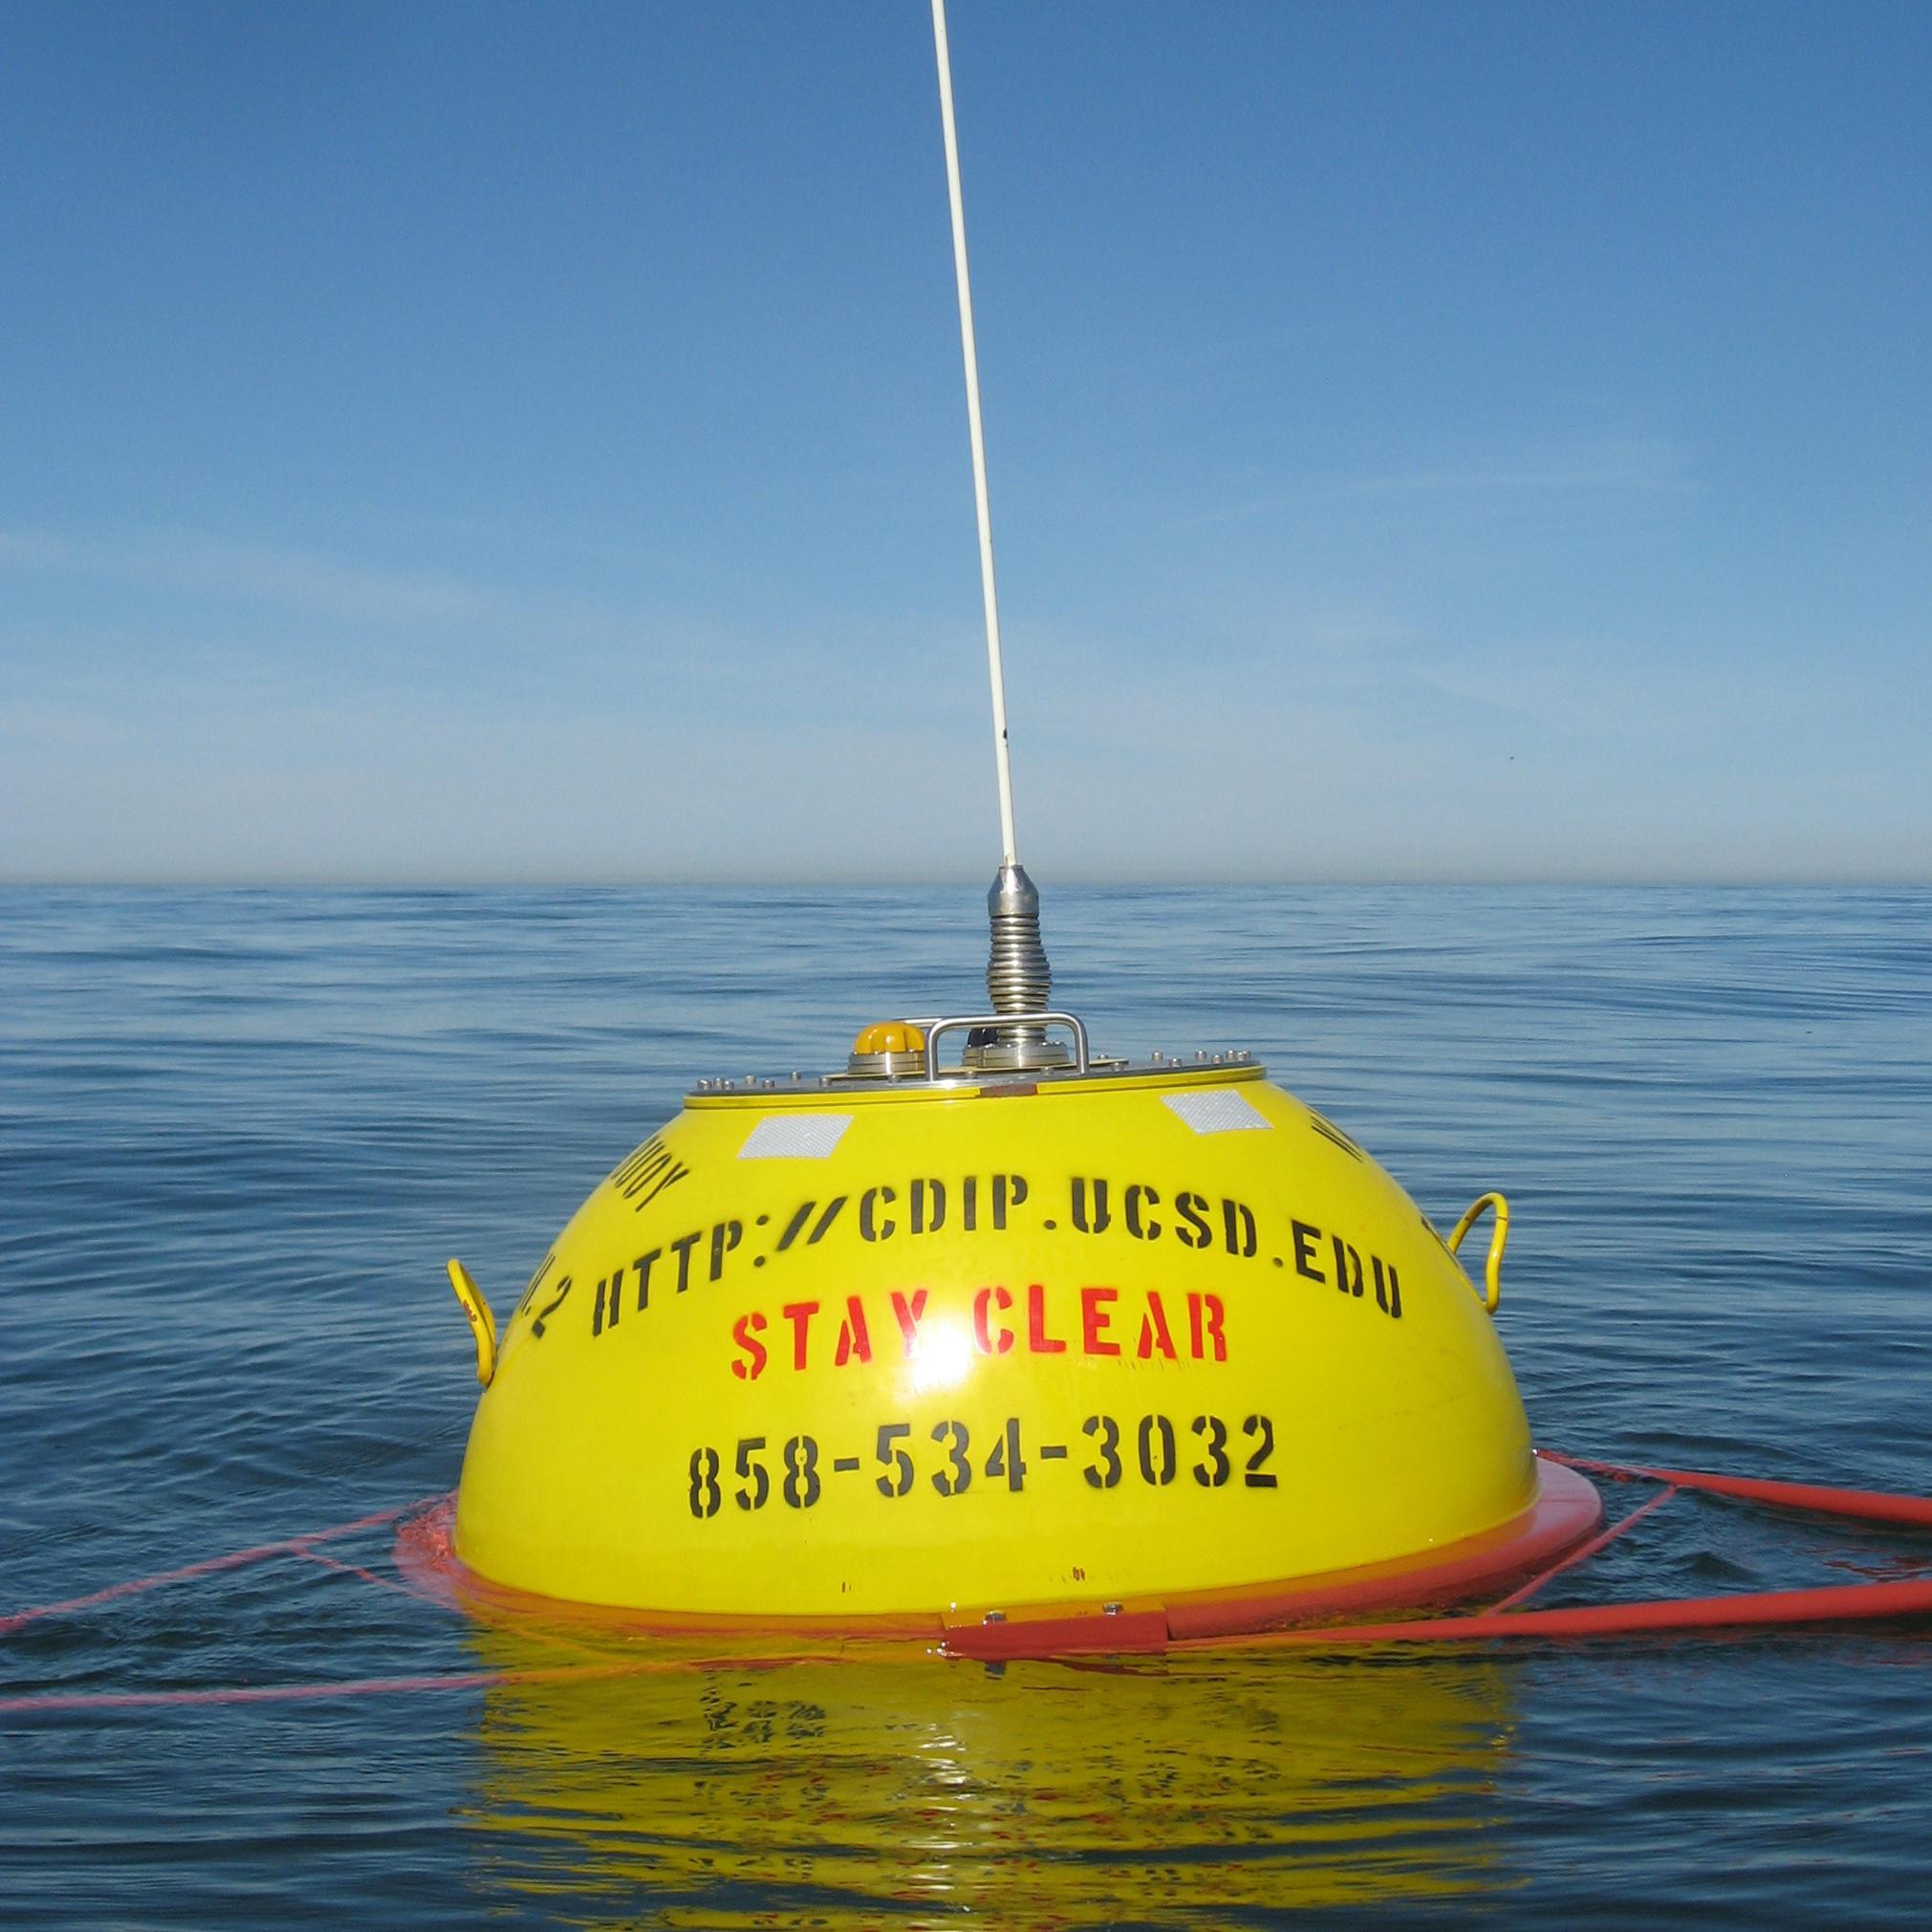
\includegraphics[height=6cm]{Figures/Chapter4/cdip.jpeg} }}%
    \caption{The two types of buoy stations moored in SNE.}
    \label{fig:example}%
\end{figure}


Information about all stations’ location characteristics and their data availability are included in Tables \ref{buoys_location} and \ref{buoys_data_availability} respectively. The anemometer height is 4.1 meters for all buoys with available wind measurements except buoys 44020 (3.8 meters) and 44039 (3.5 meters). When is needed, wind speed is adjusted at 10 meters height, assuming neutral stability of the atmospheric boundary layer, as described in \ref{WindProfile}. 


Data are available at the NDBC and CDIP websites. Directional wave spectra for buoy 44097 were downloaded from CDIP archive at THREDDS Data Server (TDS) in NetCDF format. All other geophysical parameters were downloaded from the NDBC website as \emph{.txt} files. NDBC provides an extensive description of the measurement process, the statistical analysis and quality control of the raw data, and the various error sources in \cite{Data2009}. The buoy anemometers' reported accuracy is $\pm 1m/s$ with a resolution of $0.1 m/s$. The corresponding accuracy of the SWH measurements is $\pm 0.2 m$ with a $0.1 m$ resolution. After careful examination of the quality-controlled time series, additional filtering criteria were implemented to eliminate erroneous data.


\begin{table}[H]
\begin{tabular*}{\textwidth}{c@{\hskip 0.25in}ccccc @{\extracolsep{\fill}} ccccc}
%\begin{tabular*}{\textwidth}{c @{\extracolsep{\fill}} ccccc}
\toprule
 Buoy \# &                    Location &  Lon. (deg. W) &  Lat. (deg. N) &  
 Water Depth (m) \\
\midrule
  44097 &           Block Island, RI  &    -71.127 &    40.969 &        48.16 \\
  44020 &             Nantucket Sound &    -70.279 &    41.493 &        14.30 \\
  44025 &                 Long Island &    -73.164 &    40.251 &        36.30 \\
  44017 &               Montauk Point &    -72.049 &    40.693 &        48.00 \\
  44065 &    New York Harbor Entrance &    -73.703 &    40.369 &        25.00 \\
  44039 &   Central Long Island Sound &    -72.655 &    41.138 &        27.00 \\
  44008 &      Southeast of Nantucket &    -69.248 &    40.504 &        74.70 \\
  44066 &      East of Long Beach, NJ &    -72.644 &    39.618 &        78.00 \\
  44091 &                Barnegat, NJ &    -73.769 &    39.778 &        25.60 \\
  \bottomrule
\end{tabular*}
\caption {Buoys' location, coordinates and water depth.}
\label{buoys_location}
\end{table}


 Specifically, WS data with values smaller than or equal to 0.2 m/s and SWH values lower than or equal to 0.1 meters were discarded. Previous studies \cite{Andreas2012} have used even stricter filtering criteria for the WS, recognizing that one disadvantage of the 4-blade, wind-vane sensors onboard buoys, is that they need a minimum, nonzero WS to start measuring and recording data reliably. The 0.1 meter-limit for SWH is also used by CDIP. Furthermore, data availability in terms of years of available data, as documented in Section~\ref{buoys_data_availability}, imposes the need for consistency on the final buoy time series. The final buoy datasets consist of data from 2007 until the end of 2019. Buoy time series have gaps owing to maintenance or change of the sensor payloads. The main goal was to have at least ten years of data for each buoy for consistent analysis. Previous studies have also documented that ten years of wave data are enough to characterize the seasonal variability for a specific location \cite{athanas1995}.
 
 For this reason, buoy 44091 data were used only for the validation with altimeter data. Buoy 44039 data has two disadvantages that prevented their use for other than the validation with altimeters section of this study. 


\begin{table}[H]
\centering
\begin{tabular*}{0.85\textwidth}{c@{\hskip 0.25in}cccc @{\extracolsep{\fill}} cccc}
%\begin{tabular*}{\textwidth}{c @{\extracolsep{\fill}} ccccc}
\toprule
 Buoy \# &  Distance to Coast (km)  &  Data Type & Data Availability (Years) \\
\midrule
  44097 &            41.0 &  wave only &        2009-Present \\
  44020 &            13.0 &  wind/wave &        2009-Present \\
  44025 &            42.0 &  wind/wave &        1975-Present \\
  44017 &            30.0 &  wind/wave &        2002-Present \\
  44065 &            23.0 &  wind/wave &        2008-Present \\
  44039 &            13.0 &  wind/wave &           2004-2019 \\
  44008 &           103.0 &  wind/wave &        1982-Present \\
  44066 &           121.0 &  wind/wave &        2009-Present \\
  44091 &            27.5 &  wave only &        2014-Present \\
  \bottomrule
\end{tabular*}
\caption {Buoys' distance to the closest coast and data availability depending on the type of the reported parameters and its period.}
\label{buoys_data_availability}
\end{table}


  Specifically, SWH values have a precision of one decimal number, and dominant periods are rounded to the closest integer. Data are also recorded at irregular times, which creates challenges for interpreting the results, especially compared to the other buoys' stable recording times.



\begin{figure}[H]
\centering
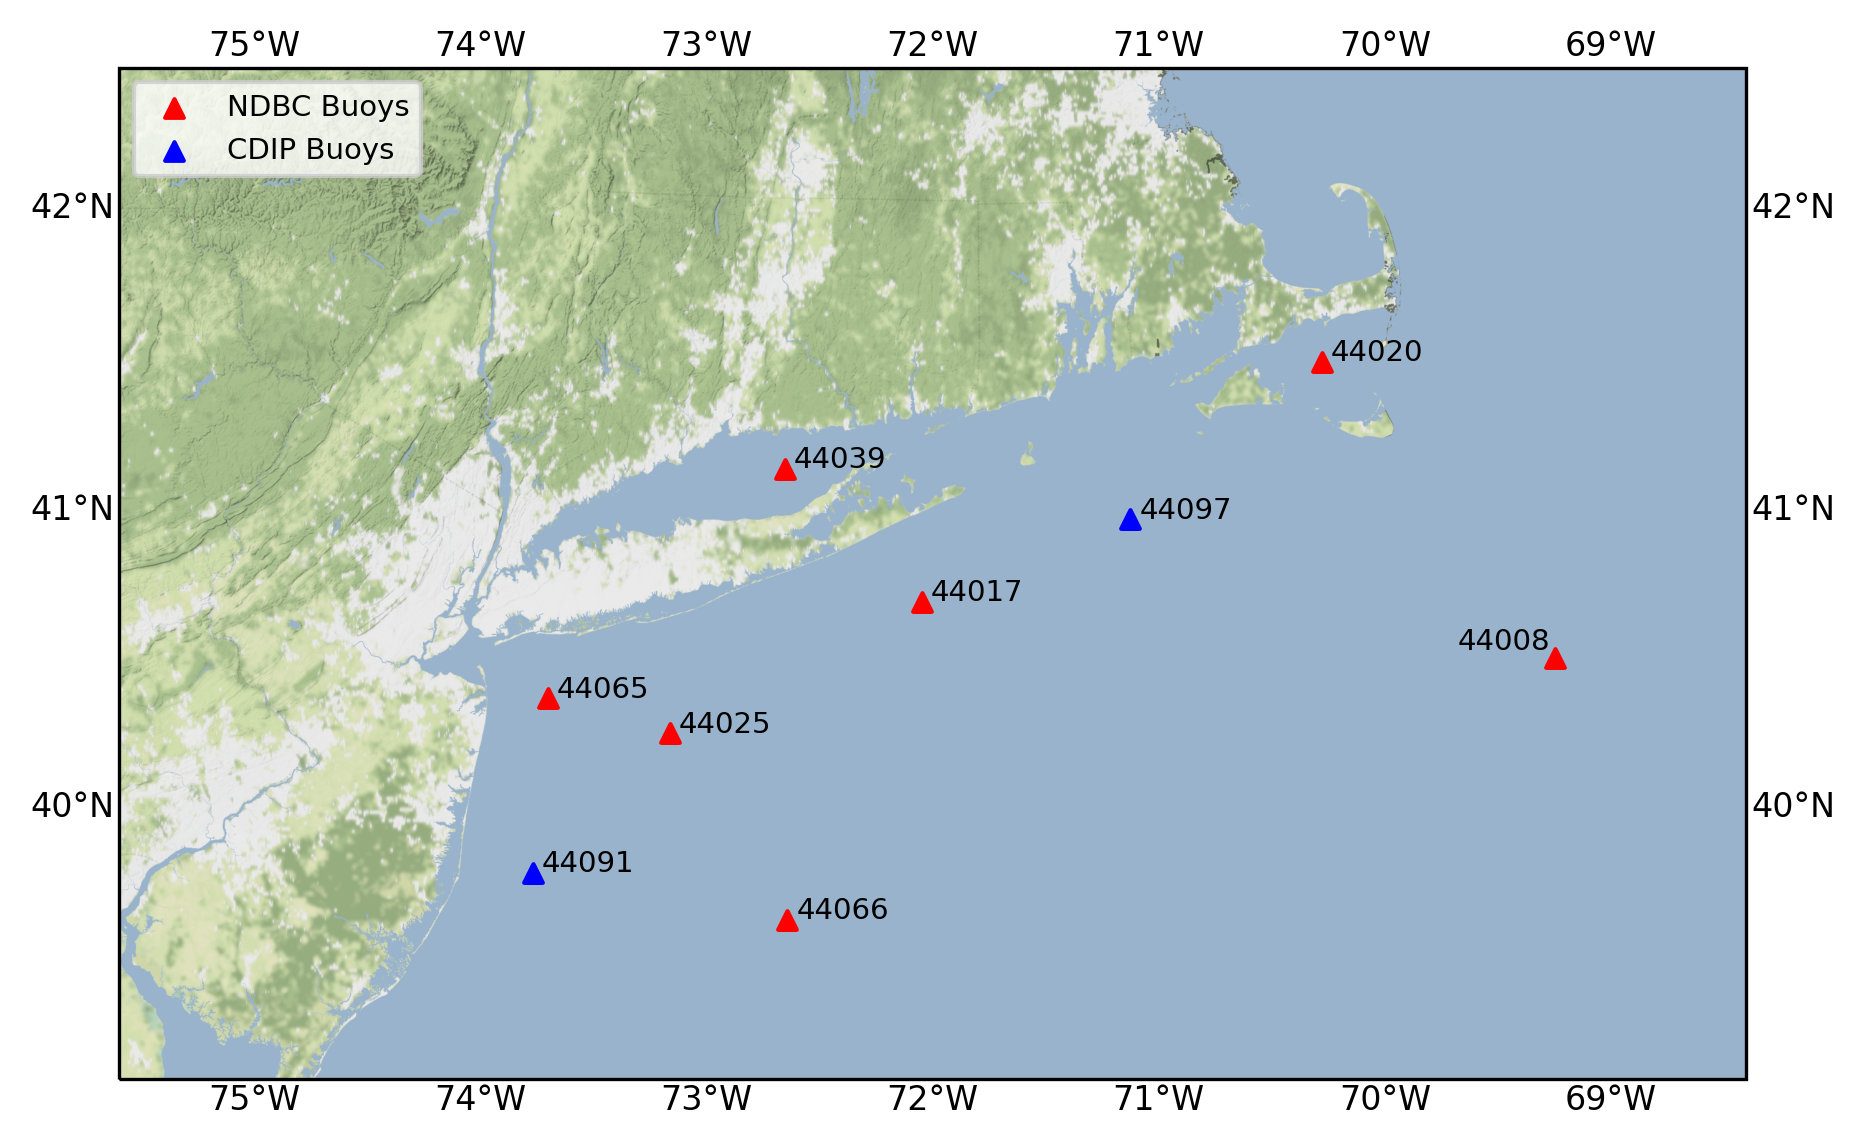
\includegraphics[width=0.95\linewidth]{Figures/Chapter4/ndbc_cdip2.png}
%\decoRule
\caption{NDBC and CDIP buoys in the SNE region.}
\label{fig:buoys_SNE}
\end{figure}


It is essential to mention the different datasets that were used and their unique characteristics. First of all, buoy payloads can record WS and wind direction in two distinct ways described in \cite{Data2009}. The first one is an 8-minute average of 1Hz observations, which leads to an hourly dataset. Data are reported at the end-of-acquisition minute, but that does not mean that the observation value includes measurements from the whole hour. This dataset was used when synchronous wind and wave observations were needed to validate altimeter data. The second one is a 10-minute average of the 1Hz observations, which is reported again at the end-of-acquisition minute. Still, the difference is that it is the average of the whole 10-minute period. This dataset is referenced as the 10-minute average dataset from now on, and it is especially useful for studying the diurnal variability and wind climate. It is also the recommended dataset for wind observations, according to BOEM for offshore wind-related studies \cite{DNVGL2018}. The 10-minute average dataset is used when wind data are processed independently, and the hourly dataset is used when combined with wave data.



Wave data are measured and reported in an entirely different way due to their more complex nature. All wave parameters are derived from the estimated energy spectra \cite{Data2009}; therefore, they are neither instantaneous nor average values of continuous observations. Wave parameters represent observations every 20 minutes. The acquisition time starts at the 20th minute of each hour and ends at the 40th. The final reported measurements are synchronized to the closest hourly wind observations. This is useful when we want to study, for example, the relationships between WS and SWH. Still, at the same time, we have to consider that the observations are not simultaneous in reality.
Data organization and preprocessing were implemented using Python \emph{Pandas} and other supplemental packages of the Python programming language. The final time series were saved as separate \emph{.txt} files for each buoy and are available for future use.


%---------------------------------------------------------------------------------------------


\subsection{Altimeter Data Collection and Organization}\label{altimeter_data}


The theoretical aspect and the distinct qualities of the satellite altimeter observations are already emphasized in \ref{AltimetryPrinciples}. This chapter will provide the necessary information regarding the altimeter datasets' characteristics, the reasons for their choice, and their actual use as input to the analysis.



\begin{table}[H]
\begin{tabular*}{0.98\textwidth}{c@{\hskip 0.25in}ccccc @{\extracolsep{\fill}} ccccc}
%\begin{tabular*}{\textwidth}{c @{\extracolsep{\fill}} ccccc}
\toprule
         &     SARAL &                  Jason 3 &      Sentinel 3A &      Sentinel 3B &        Cryosat 2 \\
\midrule
      Repeat Cycle &               35 &                       10 &               27 &               27 &              369 \\
    Frequency Band &             Ka/C &                     Ku/C &             Ku/C &             Ku/C &             Ku/C \\
 Data Availability &  03/2013- &          09/2016- &  03/2016- &  05/2018- &  07/2010- \\
 
        Instrument &           AltiKa &              Poseidon-3B &             SRAL &             SRAL &            SIRAL \\
    Operation Mode &              LRM &                      LRM &              SAR &              SAR &    LRM/SAR \\
      Product Type &              GDR &                      GDR &              NTC &              NTC &              GOP \\
  \bottomrule
\end{tabular*}
\caption {Satellite Altimeters used in this study and their characteristics.}
\label{altimeters}
\end{table}



First of all, this study's scientific context dictates the use of data from multiple altimeter missions. Currently, there are six satellite altimeters in orbit. Information about the main characteristics of each altimeter that is included in this study is provided in \ref{altimeters}. Data from the most recent altimeter mission, the Chinese HY-2B, were not used or examined. Sentinel-3A and Sentinel-3B satellites are part of the same mission, often characterized as \enquote{twins} because they have complementary orbits. They are the only satellites equipped with multiple sensors, including the radar altimeter instrument SRAL.

Satellite with ARgos and ALtiKa (SARAL-AltiKa) is a collaboration between the Centre National d'Etudes Spatiales (CNES) and the Indian Space and Research Organization (ISRO) \cite{Verron2015} with the participation of the European Organization for the Exploitation of Meteorological Satellites (EUMETSAT). This mission is unique, mainly for two reasons. SARAL-AltiKa is the first mission that takes advantage of the high-frequency Ka-band (35.75 GHz) capabilities. Specifically, its high-frequency signal means that the altimeter footprint is smaller, leading to better spatial resolution and more accurate measurements, in particular close to the coast. The disadvantage of Ka-band's high frequency is its sensitivity to water vapor and rain, leading to signal attenuation and making the atmospheric corrections even more challenging \cite{Bonnefond2018, Tournadre2009}. SARAL-AltiKa is also unique because it was launched using the same orbit and ground tracks as its predecessor mission, ERS, from March 2013 until July 2016. From July 4, 2016, it has entered its second phase, which is called the drifting phase or SARAL-DP. Since then, SARAL-AltiKa does not maintain its altitude; therefore after each repeat cycle, its ground tracks are no longer passing from the same location as the previous, but they \enquote{drift} a few kilometers. The mission agencies made this decision to preserve a few more years of its lifetime. It has been proven that it is possible to maintain good mesoscale sampling even without keeping the same altitude for the satellite \cite{Dibarboure2018}.


The Jason 3 mission involves CNES, the National Aeronautics and Space Administration (NASA), EUMETSAT, and the National Oceanic and Atmospheric Administration (NOAA). It is the successor of Jason 2, and it was launched on January 17, 2016. Jason 3 entered its calibration and validation phase on February 19, 2016, when it also started measuring and reporting data. Its primary instrument, the Poseidon-3B altimeter, sends and receives its impulses in Low-Resolution Mode (LRM), and it operates in Ku-band (13.575 GHz). Jason 3 is also unique because it has the highest temporal resolution and the lowest spatial resolution of all the altimeters. Every repeat cycle covers ten days, and every ascending or descending along-track is at an approximately 2.8 degrees distance from the closest. The instruments onboard Jason 3, which are also common to satellites that include altimeters, are shown  Figure~\ref{fig:jason3_payload}.

Sentinel 3 mission is organized and implemented by the European Space Agency (ESA) and EUMETSAT. Satellite altimetry is one of its main objectives, but not the exclusive. Its payload also includes instruments that measure and record Sea Surface Temperature (SST) and Ocean Colour data that are equally important to the geophysical parameters derived from the radar altimeter. So far, Sentinel 3 is comprised of two satellites, Sentinel 3A and Sentinel 3B. Sentinel 3A launched on February 2016 and Sentinel 3B on April 2018. They are often characterized as the \enquote{twin mission} because their along-tracks are complimentary to increase spatial coverage. Both satellites are equipped with the same payloads; hence they will be referenced in this study as Sentinel 3. Sentinel 3 SRAL altimeter sends and receives its impulses in Ku-band. It is also worth mentioning that it is the first mission that operates in SAR (or delay-Doppler \cite{KeithRaney1998})  mode exclusively, even if it can function in both SAR and LRM modes. As a result, only the across-track resolution of its effective footprint is still pulse-limited because the along-track resolution is increased and constrained to 300 meters. Conventional altimetry operates in low-resolution mode, which is pulse-limited on both the across and the along-track directions. SRAL altimeter’s received pulses can also be processed in Pseudo-Low Rate Mode (PLRM) and produce LRM-like waveforms when operating in SAR mode. Still, PLRM's estimates are noisier and have worse performance in coastal regions \cite{Nencioli2019}. In this study, only SAR mode data are used and evaluated.

Cryosat 2 is an ESA mission launched on April 2010, and its primary objective is to monitor the Arctic sea ice extent. It is a pioneer altimeter mission because it is the first-ever to operate in SAR mode. Specifically, the SIRAL altimeter onboard Cryosat 2 can operate in three modes: LRM, SAR, and SAR Interferometry (SARIn). Generally, SIRAL operates like a traditional altimeter in LRM mode. SAR processing mode is available for a few oceanographic areas, specific for each cycle. SARin is only available for the ice sheet margins and over mountain glacier regions. Therefore, Cryosat 2 data used in this study are LRM-processed with very few exceptions that are processed using the SAR waveforms. Cryosat 2 has the most extended repeat cycle (369 days) with an approximately 30-day subcycle covering a specific region of interest. It is also worth mentioning that its orbit does not repeat after completing every cycle, unlike every other conventional altimeter mission, which makes it unique in that regard.

For each mission, there are three types of dataset files available: a reduced dataset that contains only the 1Hz data, a native or standard including both the 1Hz and the 20Hz parameters, and an expert or enhanced sensor product that includes the full waveforms. Only the native dataset was collected, organized, and used for this study. 


\begin{figure}[H]
\centering
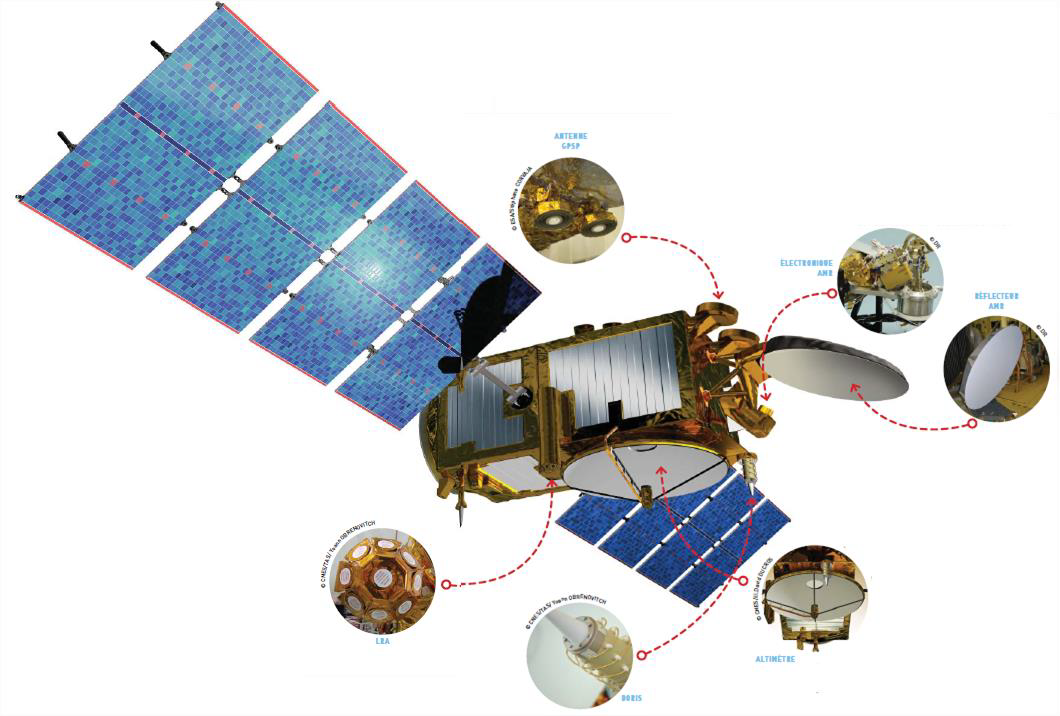
\includegraphics[width=0.95\linewidth]{Figures/Chapter4/jason3_payload.png}
%\decoRule
\caption{The main components of Jason 3 payload including the radar altimeter Poseidon-3B (center), the Advanced Microwave Radiometer (AMR, upper center) and the radio positioning DORIS system for the precise determination of its orbit (lower center). Other instruments include a Laser Reflector Array (LRA) used for the calibration of the orbit determination system (lower left) and a precision Global Positioning System Payload (GPSP) antenna (upper left). These components are common to all satellites that contain altimeter instruments. Derived from: \cite{Jason32018}}
\label{fig:jason3_payload}
\end{figure}



Besides, every altimeter mission has a family of three distinct Level 2P (processed) product types, distinguished by increasing latency and accuracy. This family of products is often called Geophysical Data Records (GDR). Near Real-Time (NRT) or Operational GDR (OGDR) products are mainly useful for the operational community. They are disseminated only a few hours after the initial waveforms are received, but they may contain outliers. Short Time Critical (STC) or Interim GDR (IGDR) products have additional auxiliary data used in the processing, and they are provided a couple of days after the NRT products. The third product type is the Non-Time Critical (NTC), or GDR, and the only one used in this study. For Cryosat 2, this product type is called Geophysical Ocean Product (GOP) to distinguish it from the ice processors’ GDR dataset. LRM products are followed by an additional M letter (GOPM) and SAR products with an R (GOPR). These products are delivered typically one month or two months after data acquisition with more precise orbit determination and atmospheric corrections. It incorporates additional auxiliary/ancillary data with lower errors.

There are different dataset standards throughout the lifetime of each altimeter. Generally, the initial standard uses the waveform retracking algorithms and geophysical/atmospheric corrections of the calibration/validation (Cal/Val) phase. Then, depending on the instrument's skills and contemporary research developments, the initial standards are updated one or two times during every altimeter's lifetime. Specifically, in this study, Jason 3 GDR-T data are used from February 2016 until September 2016. From September 2016, the GDR-D version is used. The most recent, GDR-F version of SARAL-AltiKa data is used for its first phase (March 2013 until July 2016) and also for the period from November 2019 until July 2020. For the intervening period, the previous (GDR-T) version is used because it is not disseminated yet on the AVISO \emph{ftp} server in its entirety.

Quality control is critical during the preprocessing stage. Editing criteria should be implemented on Level 2 data to filter outliers or erroneous data and keep only the valid observations before their use in the analysis. The two primary sources of the suggested editing criteria are every mission's data handbook \cite{Bronner2013, ESA2019, EUMETSAT2017, Mertz2017, Jason32018}, and the Quality Assessment Reports (QAR) that accompany the data files after the completion of each cycle. Generally, the discarded observations are not extensive due to the high data quality from the current missions. As already discussed, each altimeter has its unique features. For example, SARAL-AltiKa’s Ka-band is more sensitive to rain and water vapor. Simultaneously, it is expected to provide more observations with higher accuracy close to the coast because of its smaller wavelength and effective footprint. These characteristics are also reflected in the valid altimeter data for each mission. It is the user's responsibility to select the suitable editing criteria according to the application. For this study, we use the official mission handbooks and QAR guidelines to filter suspect or erroneous Level 2 altimeter data.

Although there are multiple sources of satellite altimetry data, SARAL-AltiKa and Jason 3 GDR data were downloaded from the \href{https://aviso-data-center.cnes.fr/}{Aviso-CNES Data Center} website, Sentinel 3 NTC data were downloaded from the \href{https://coda.eumetsat.int/#/home}{EUMETSAT Coda} website, and Cryosat 2 data were downloaded using ESA’s Cryosat User Tool (CUT).

For the preprocessing stage, NetCDF data files were input, subsetted, filtered using Python \emph{xArray} \cite{Hoyer2017} package, and the final, quality-controlled data were written to single, \emph{.txt} files using Python \emph{Pandas} \cite{McKinney2010} to be available for future use.


%----------------------------------------------------------------------------------------

\section{Spatio-temporal collocation}\label{collocation}


The satellite altimeter products consist of point observations that are representative of the nadir-pointing sensor’s footprint center. We have previously discussed that the altimeter's effective footprint cannot be considered a single point, though. It has a radius that is not constant and changes with respect to the sea state. This is also important when we want to compare altimeter measurements' accuracy against the buoys, which are stations in point locations.

A review of the different validation approaches, terminology, and metrics to assess the quality of satellite observations is available in \cite{Loew2017}. Validation is a process that requires the determination of specific criteria by the user to accomplish two primary goals. First of all, there should be limits to the two datasets' proximity both in space and time. The process of applying these limits is called spatiotemporal collocation and results in the final datasets with the collocated observations to compare. Indeed, the validation of altimeter against buoy observations is sensitive primarily to selecting the collocation or sampling radius and secondarily to the chosen time window \cite{Hwang1998}. It has been documented that a reduced sampling radius or closer proximity of the two observations in space leads to smaller absolute differences between the two collocated values \cite{Monaldo1988}. Traditionally, for global scale validation of 1 Hz altimeter data, a sampling radius of 50 or 25 kilometers and a time window of 30 or 60 minutes is selected. The data are again quality-controlled to remove possible outliers. The individual measurements are then straightforward or weighted averaged to compare with the buoy observations because they are considered simultaneous with a spatial distance of 6 to 7 kilometers \cite{Durrant2009, Queffeulou2004, Yang2019}. The selection of a suitable sampling radius becomes challenging when approaching a coastal region due to the land contamination of the waveforms and the number of available stations. The former is discussed in \ref{AltimetryPrinciples}, and the latter is the second goal we must achieve, the statistical significance of the results. Validation is often a compromise between the two, and selecting the appropriate sampling radius and time window depends on the application.


There are inherent sources of measurement error in both types of observations. The accuracy of WS and SWH measurements from buoy sensors is reported in \ref{buoy_observations}. On the other hand, the challenges of coastal altimetry are explained in \ref{AltimetryPrinciples}. The primary sources of inaccuracy in altimeter measurements include estimating parameters like the backscatter coefficient or the altimeter range from the waveform retracking and the empirical nature of the algorithms used to calculate the final geophysical parameters (SSH, SWH, WS). Hence, instrumental errors are the first source of uncertainty when comparing two different measurement systems' observations. Even if the two measurement systems had zero or identical uncertainty, their comparison would still be challenging due to their diverse spatial and temporal sampling. In other words, we need to consider how close are the observations in space and time due to the wind and wave variability in multiple spatial and temporal scales. Furthermore, we also need to take into account the sampling variability of the two types of observations. Specifically, the reported observations from buoys as described in \ref{buoy_observations} are temporal averages, whereas the 1Hz altimeter values are considered instantaneous.


This study aims to validate wind speed and significant wave height measurements from altimeters with buoys in the SNE. There are limited buoy stations in this domain, as described in \ref{buoy_observations}. At the same time, most of the stations are located closer than 50 kilometers from the coast, which is a choice of a limit for similar studies \cite{Yang2019}. In contrast, data with proximity to land are not discarded in other studies to retain a larger sample size \cite{Queffeulou2004}. Therefore, the limits selection is a compromise between accuracy and statistical significance. Specifically, a 10-kilometer sampling radius around and a time window of 30 minutes before and after each buoy observation are chosen. The time window is reduced to 15 minutes for the CDIP waverider buoys, which have a more frequent recording of data (every 30 minutes). These criteria fulfill the first goal since the closest distance to the coast is 13 kilometers for buoys 44039 and 44020; hence, we can find a considerable amount of collocated measurements from altimeters in these locations, and we avoid erroneous data due to land contamination. Still, the sample size of collocated data gets smaller as we are approaching the coast. On the other hand, the validity of altimeter observations inside semi-enclosed basins like, for example, the Long Island Sound or in areas surrounded by land and islands like the Nantucket Sound is one of this study's goals. Besides, it has been documented that the compared observations' spatial proximity plays a larger role than the temporal proximity \cite{Hwang1998, Monaldo1988}. For the reader’s convenience, we call the two buoys mentioned above as \enquote{sheltered}, the buoys which are closer than 50 kilometers from land as \enquote{coastal}, and the ones with a distance over 50 kilometers off the coast as \enquote{open ocean} buoys. The results presented in \ref{validation_SNE} are all statistically significant, and the sample size of the collocated dataset is adequate for their interpretation. We examined the option to increase the sampling radius around the open ocean buoys. Still, we decided to be consistent with the coastal and sheltered buoys and compare them using the correlation coefficient. The 30-minute time window was selected because the hourly buoy WS and SWH datasets are used for the validation and also taking into account the buoy reporting times described in \ref{buoy_observations}.


The exact, great-circle distance given the buoys and the altimeter observations coordinates were calculated using the haversine formula \ref{eqn:haversine}, where $\theta_{1}$, $\theta_{2}$ are the latitude and $\phi_{1}$, $\phi_{2}$ are the longitude coordinates of the two locations in radians. The time difference is calculated using the dates and times of the reported observations. Once the sampling radius and time window limits are applied, the collocated dataset is created. The average calculated distance is 7 kilometers. This distance is acceptable, especially when the altimeter measurement principles and the effective footprint (2-7 kilometers depending on sea state) is considered. By selecting a 10-kilometer radius, one or two collocated 1Hz altimeter observations correspond to every buoy value. In the case of two collocated altimeter observations, the first one is located north and the second south of the buoy's location. The average of the two values is calculated and then compared with a single buoy measurement. 


\begin{equation}
D(\theta,\phi) = 2 \cdot \arcsin{\left(\sqrt{\sin^{2}{\left(\frac{\theta_{2}-\theta_{1}}{2}\right)} + \cos{\theta_{1}} \cdot \cos{\theta_{2}} \cdot \sin^{2}{\left(\frac{\phi_{2}-\phi_{1}}{2}\right)}}\right)}
\label{eqn:haversine}
\end{equation}


The comparison of the two datasets was performed with Ordinary least squares linear regression. The slope and the intercept of the linear model fit are reported. Evaluation of the comparison is realized by calculating commonly used pairwise metrics \cite{Durrant2009, Yang2019} :


\begin{equation}
Bias = \frac{1}{N} \sum_{i=1}^{N} \left(A_{i}-B_{i}\right)
\label{eqn:bias}
\end{equation}

\begin{equation}
RMSE = \sqrt{\frac{1}{N} \sum_{i=1}^{N} \left(A_{i}-B_{i}\right)^2}
\label{eqn:rmse}
\end{equation}

\begin{equation}
SI = \frac{\sqrt{\frac{1}{N} \sum_{i=1}^{N} \left[ \left(A_{i}-\bar{A}\right) - \left(B_{i}-\bar{B}\right) \right]^2 }}{\bar{B}}
\label{eqn:scatter_index}
\end{equation}

\begin{equation}
R = \frac{\sum_{i=1}^{N} \left(A_{i}-\bar{A}\right) \left(B_{i}-\bar{B}\right) }{\sqrt{ \sum_{i=1}^{N}  \left(A_{i}-\bar{A}\right)^2 \left(B_{i}-\bar{B}\right)^2}}
\label{eqn:correlation}
\end{equation}

Bias is used to assessing the systematic errors or differences between the two datasets, RMSE is the Root Mean Square Error, SI is the scatter index and R is the Pearson’s Correlation Coefficient. $A_{i}$ are the altimeter values, $B_{i}$ are the buoy values,  $\bar{A}$, $\bar{B}$ represent their corresponding mean values, and  N is the collocated dataset sample size.

All calculations described above are computationally intensive due to the size of the datasets. Python library \emph{NumPy} \cite{Harris2020} and its vectorized operations helped to efficiently optimize all computations. Regression analysis was performed, and evaluation statistics were calculated using the Python libraries \emph{Scikit-learn} and \emph{SciPy}  \cite{Varoquaux2015, Virtanen2020}.


%---------------------------------------------------------------------------


\section{Variogram Modeling and Kriging Interpolation}\label{variogram_kriging}


Variogram modeling is defined by the variogram or semivariogram estimator function, which describes a variable's correlation in space. The variogram estimator is then crucial to predicting a particular variable's values at unobserved locations and obtain information on these predictions' accuracy.

The classical variogram estimator is:


\begin{equation}
\gamma(h) = \frac{1}{2N(h)} \sum^{N(h)}_{i=1} \left(z(x_{i})-z(x_{i}+h) \right)^{2}
\label{eqn:variogram_estimator}
\end{equation}

There are also other, more robust estimator functions that we can use like, for example, the Cressie \cite{Cressie1980}, the Dowd \cite{Dowd1984}, or the Genton \cite{Genton1998} estimators. This equation's parameters will be explained based on an example using satellite altimeter data on the SNE region for the winter 2019 season. The variogram estimates (blue dots) and the corresponding model (green line), which best fits the data, are presented in Figure~\ref{fig:variogram_model}.

First of all, $z(x_{i})$ is the observed value at point x and $z(x_{i}+h)$ is the observed value at a distance h from point x. This distance is called the lag interval. Lag intervals result from a process called binning, in which we classify pairs of observations in groups based on their separation distance. Figure~\ref{fig:variogram_model} shows five groups of multiples of the first lag distance of 0.4 degrees until a maximum lag distance of 2 degrees, which can be selected by the user. \emph{N(h)} is the number of observation pairs for each lag interval and is represented by the red histogram bars. With this process, all pairs of observations are given specific values of semivariances $\gamma(h)$ on the y-axis. We use the term semivariance due to the pairs of point observations. Hence, the semivariances represent variance per observation.


\begin{figure}[H]
\centering
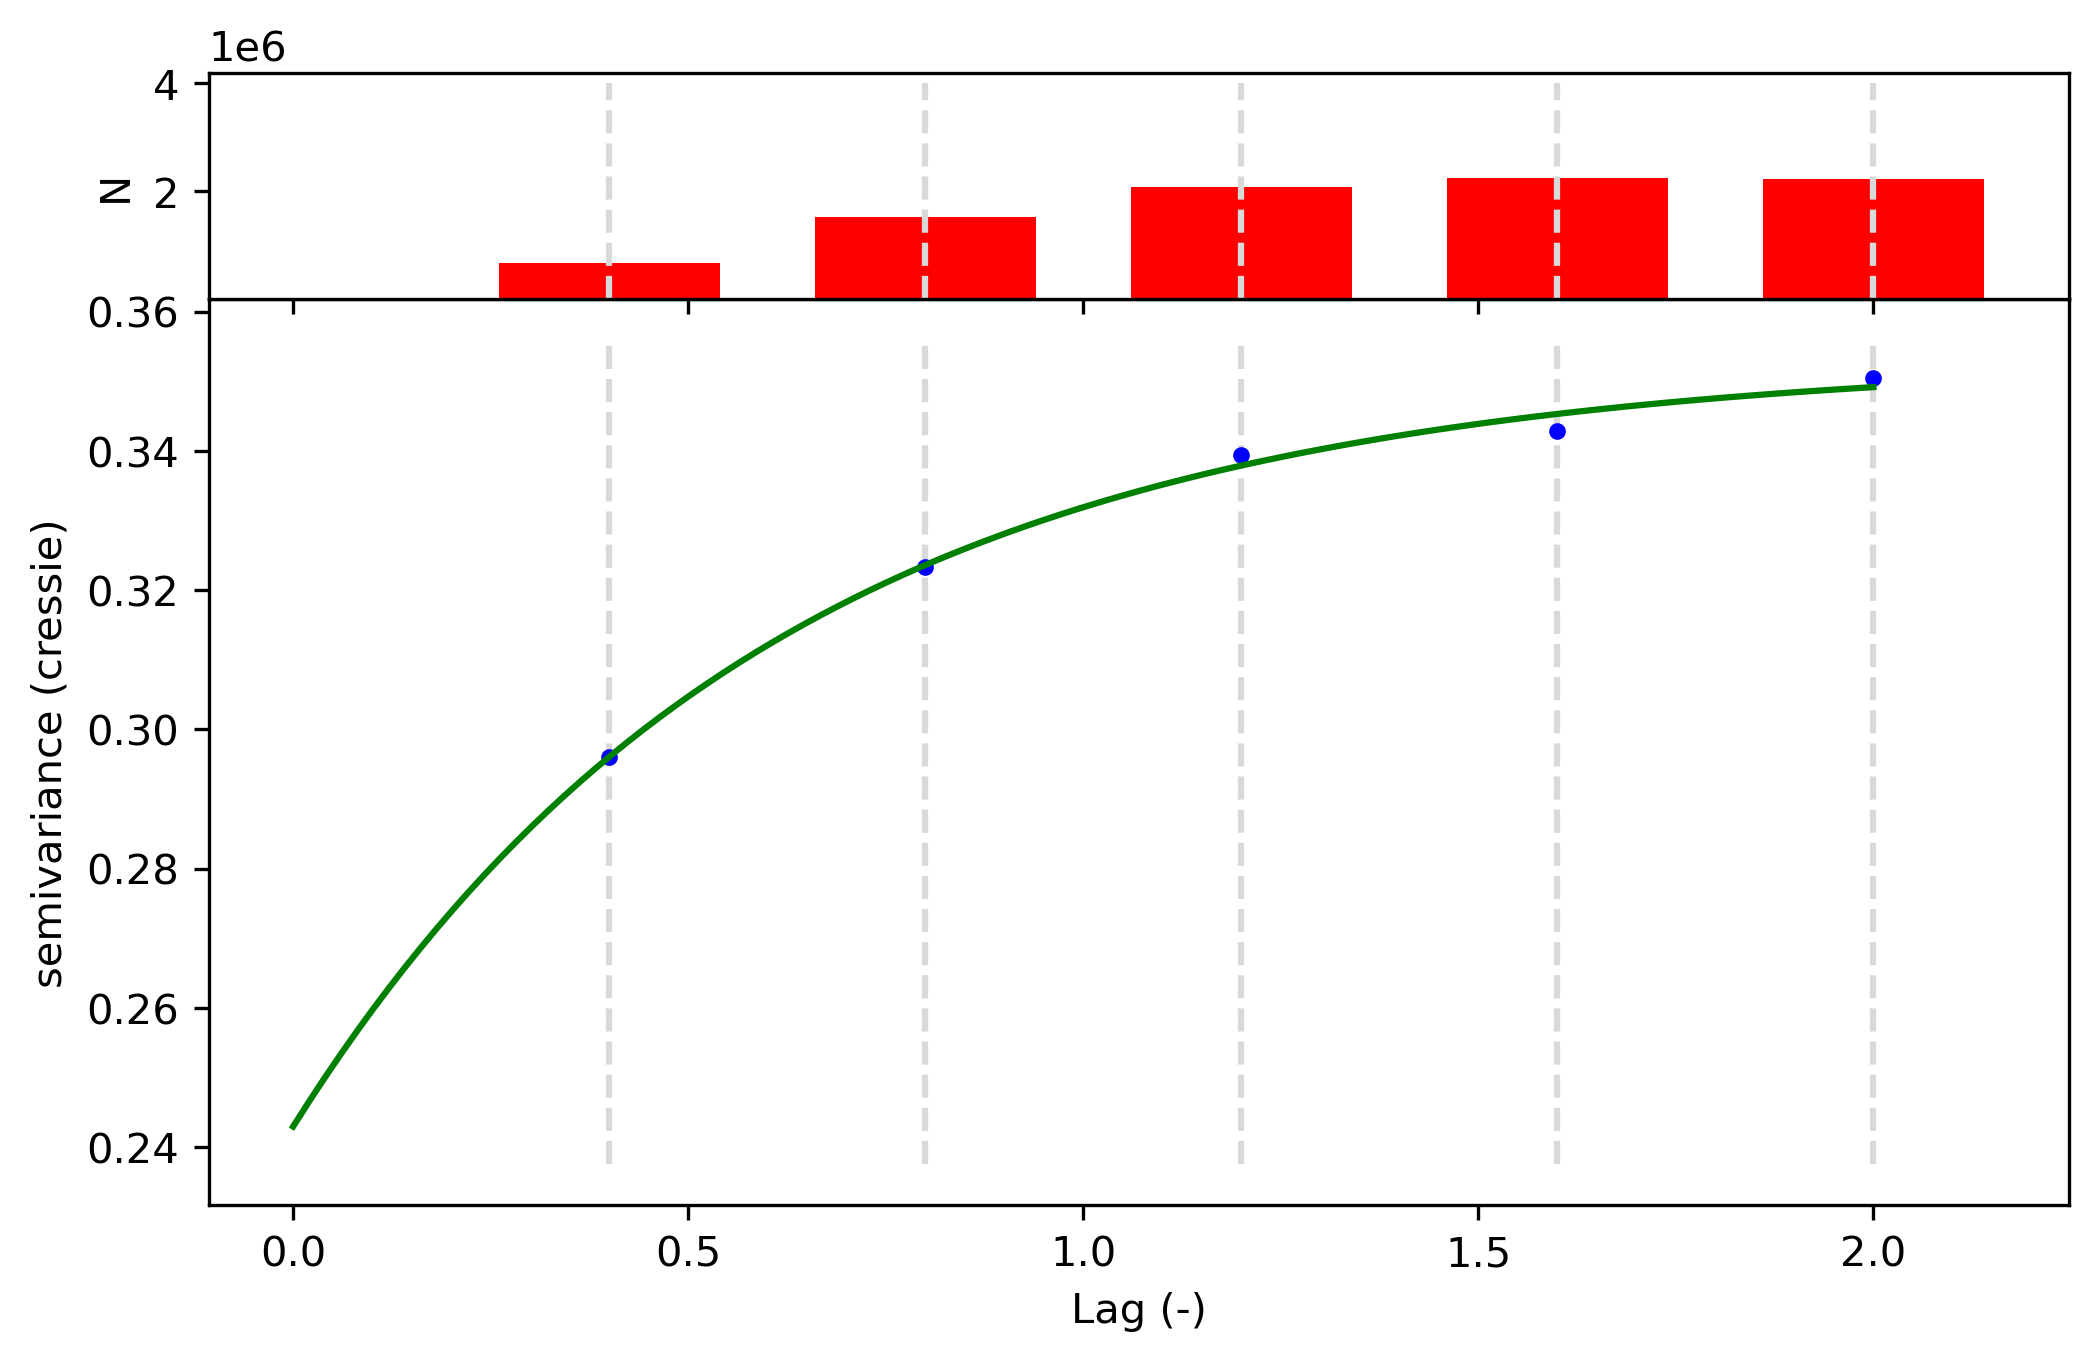
\includegraphics[width=0.8\linewidth]{Figures/Chapter4/variogram_swh2018.png}
%\decoRule
\caption{Variogram model for the satellite altimeter $H_{s}$ data for the Winter 2019 season.}
\label{fig:variogram_model}
\end{figure}


There are three fundamental parameters defined by the variogram. The first one is the sill, a variance plateau that is reached with increasing lag intervals. The sill has a value of approximately 0.11 in Figure~\ref{fig:variogram_model}. Specifically, it is called the partial sill in this example because there is an additional nugget effect, the second fundamental parameter of the variogram. The nugget can be observed as the y-intercept on the variogram (approximately 0.24 in Figure~\ref{fig:variogram_model}). It represents the minimum variance value, which exists even in zero lag interval due to small scale variations that are not captured by the large lag intervals \cite{Trauth2006}. When the nugget effect is present, the full sill is equal to the partial sill with the nugget's addition. The third variogram parameter is the range, defined as the lag distance at which the variogram reaches the sill or the partial sill if there is a nugget effect.  



Once the variogram estimator function is defined, we can fit the variogram model. Certain functions can only be used as variogram models. The most commonly used is the spherical model. Other models used to fit the variogram estimator function are the exponential, linear, Gaussian, and Matern models. Both Python libraries that were used in this study, \emph{PyKrige} \cite{Murphy2020} and \emph{SciKit GStat} \cite{Malicke2020}, provide multiple variogram estimators and models. The evaluation of each combination is performed with metrics like the correlation coefficient and RMSE and the variogram model visualization.

It is essential to mention that to perform kriging interpolation, we need to consider that the observations have to be Gaussian distributed before modeling the variogram. The variogram is sensitive to strong positive skewness resulting in higher semivariance values. Hence, if the data distribution has a long tail to the right, it is common to transform it into Gaussian using the Box-Cox transformation. An example is Figure~\ref{fig:boxcox_transform}A showing the distribution of the altimeter $H_{s}$ dataset for winter 2019. Figure~\ref{fig:boxcox_transform}B shows the distribution after the Box-Cox transformation.


\begin{figure}[H]
\centering
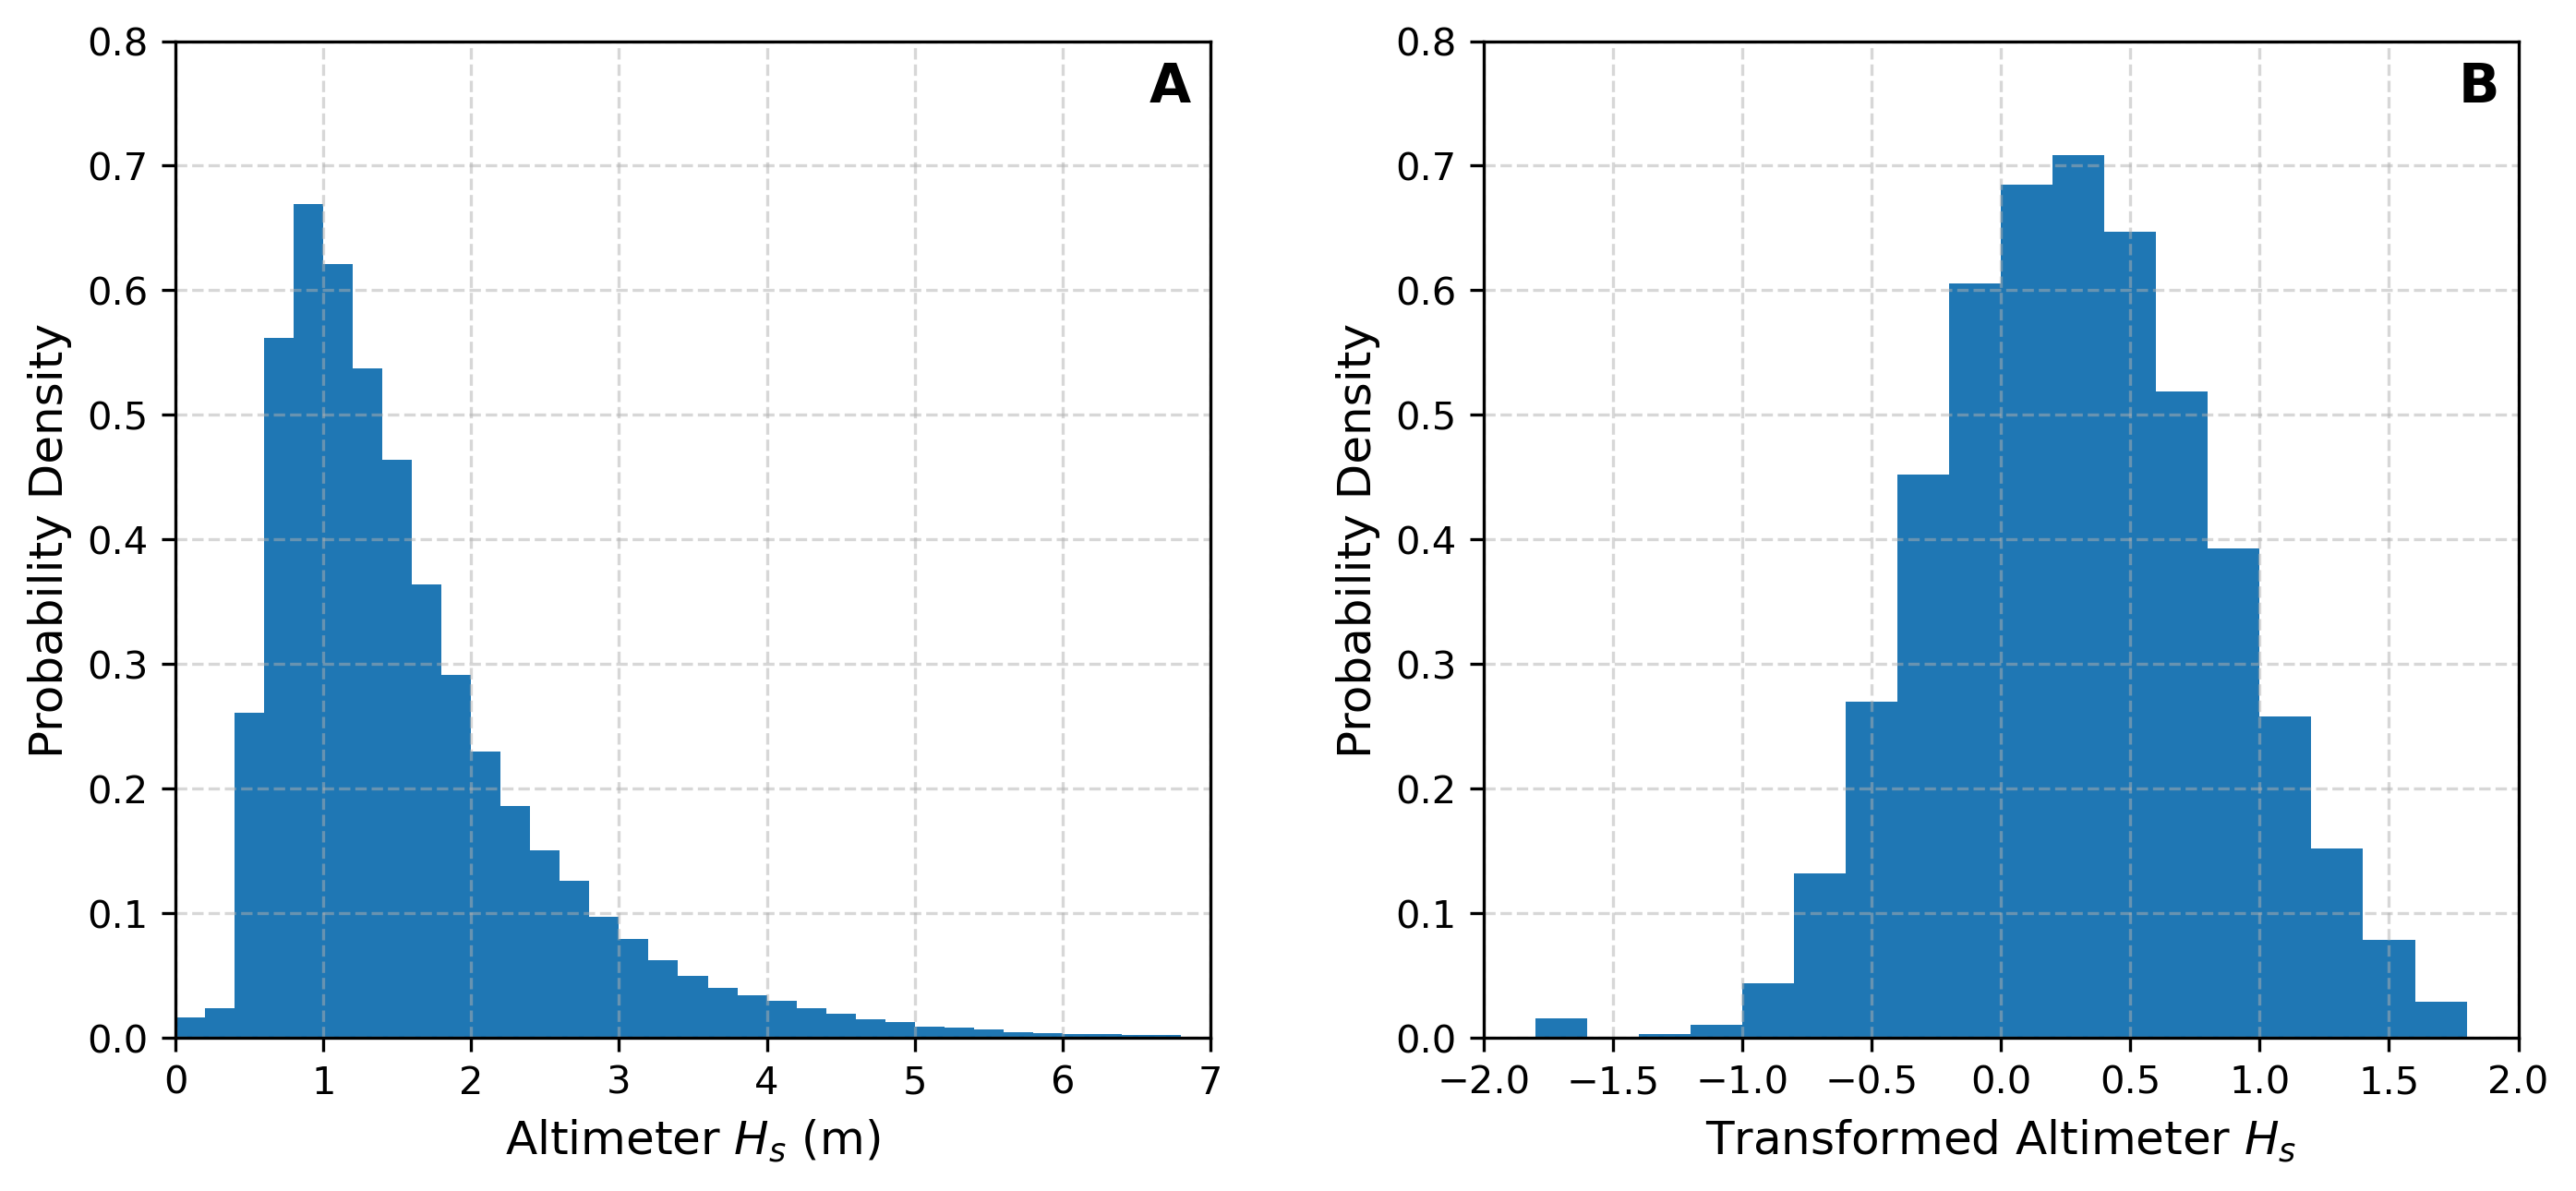
\includegraphics[width=0.85\linewidth]{Figures/Chapter4/altimeter_transobs_swh.png}
%\decoRule
\caption{A. The original altimeter $H_{s}$ distribution for the Winter 2018 season and B. The transformed to normal distribution for the same dataset.}
\label{fig:boxcox_transform}
\end{figure}



After transforming the data and modeling the variogram, we can interpolate the point observations to a regular grid. There are several types of kriging interpolation, but the most common and the one that is used herein is ordinary kriging of point observations. It is based on the assumption that we do not know the variable mean. First, the weighted average of neighboring observations is calculated to estimate a variable's value in an unobserved location.

\begin{equation}
\hat{z}(x_{0}) = \sum^{N}_{i=1} \lambda_{i} z(x_{i})
\label{eqn:kriging_interp}
\end{equation}


$\lambda_{i}$ are the kriging weights, and the condition that applies to them is that their sum should be equal to 1 to ensure that the estimates are unbiased. The value at each grid point is accompanied by a predicted error value or the kriging variance $\sigma^{2}(x_{0})$, and it is connected both with the variogram and the kriging weights.

\begin{equation}
\sigma^{2}(x_{0}) = 2 \sum^{N}_{i=1} \lambda_{i} \gamma(x_{i},x_{0}) - \sum^{N}_{i=1} \sum^{N}_{j=1} \lambda_{i} \lambda_{j} \gamma(x_{i},x_{j})
\label{eqn:kriging_error}
\end{equation}

$\gamma(x_{i},x_{j})$ is the semivariance between $x_{i}$, $x_{j}$ and $\gamma(x_{i},x_{0})$ is the semivariance between $x_{i}$ and the point we want to estimate $x_{0}$. The second condition that should be satisfied for kriging interpolation is that the estimated weights have to minimize the variances on equation~\ref{eqn:kriging_error}. This optimization is accomplished mathematically with the inclusion of Lagrange multipliers. After the solution of a system of equations, we estimate the kriging weights. Then, we estimate the variable values at the unobserved grid point locations using \ref{eqn:kriging_interp} and the kriging variance for each grid point is calculated by:


\begin{equation}
\sigma^{2}(x_{0}) = 2 \sum^{N}_{i=1} \lambda_{i} \gamma(x_{i},x_{0}) + \psi(x_{0})
\label{eqn:kriging_variance}
\end{equation}


Finally, we need to emphasize the impact of the observations' relative distance on weights. First of all, nearby point observations to the unobserved locations have higher corresponding values of weights. However, when these points are concentrated in specific areas, their weights are lower with respect to those for isolated observations. Besides, increasing nugget variance in the variogram means that the weights of nearby points become smaller.


%----------------------------------------------------------------------------------------

